\documentclass[10pt,UTF8]{ctexart}
\usepackage{amsmath}
\usepackage{graphicx}
\usepackage{hyperref}
\usepackage{underscore}
\hypersetup{ colorlinks=true, linkcolor=blue, filecolor=gray, urlcolor=blue, citecolor=blue, }
\title{Import系统}
\author{ZhangXu}
\begin{document}
\maketitle
\part{The import system}
通过importing过程,一个模块中的Python代码可以访问另一个模块中的代码。import语句是调用导入机制的最常用方法,但它不是唯一的方法。 \textbf{importlib.import_module()和内置__import__()}等函数也可用于调用导入机制。\\
\indent import语句结合了两个操作;它搜索命名模块,然后将搜索结果绑定到本地范围中的名称。import语句的搜索操作定义为使用适当的参数调用__import__()函数。__import__()的返回值用于执行import语句的名称绑定操作。有关该名称绑定操作的确切详细信息,请参阅import语句。\\
\indent 对__import__()的直接调用仅执行模块搜索,如果找到则执行模块创建操作。
虽然可能会发生某些副作用,例如导入父包,以及更新各种缓存(包括sys.modules),只有import语句执行\textbf{名称绑定}操作。\\
\indent 执行import语句时,将调用标准的builtin __import __()函数。调用导入系统的其他机制(例如importlib.import_module())可以选择绕过__import __()并使用自己的解决方案来实现导入语义。\\
\indent 首次导入模块时,Python会搜索模块,如果找到,它会创建一个module object(see types.ModuleType),并对其进行初始化。如果找不到指定的模块,则引发ModuleNotFoundError。 Python在调用导入机制时实现了搜索命名模块的各种策略。可以使用以下部分中描述的各种钩子来修改和扩展这些策略。
\paragraph{Changed in versio 3.3:}导入系统已更新为完全实现PEP 302的第二阶段。不再有任何隐式导入机制 - 完整导入系统通过sys.meta_path公开。此外,还实现了本机命名空间包支持(参见PEP 420)。
\section{importlib}
importlib模块提供了一个丰富的API,用于与导入系统进行交互。例如,importlib.import_module()提供了一个推荐的,比内置的__import__()更简单的API,用于调用导入机制。有关其他详细信息,请参阅importlib库文档。
\section{Packages}
Python只有一种类型的模块对象,所有模块都属于这种类型,无论模块是用Python,C还是其他方式实现。为了帮助组织模块并提供命名层次结构,Python有一个包的概念。\\
\indent 您可以将包视为文件系统上的目录,将模块视为目录中的文件,但由于包和模块不需要源自文件系统,因此不要太习惯。出于本文档的目的,我们将使用这种方便的目录和文件类比。与文件系统目录一样,包是按层次结构组织的,包本身可能包含子包以及常规模块。\\
\indent \textbf{重要的是要记住所有包都是模块,但并非所有模块都是包}。换句话说,包只是一种特殊的模块。具体来说,任何\textbf{包含__path__属性}的模块都被视为包。所有模块都有一个名称。子包名称与其父包名称分开,类似于Python的标准属性访问语法。因此,您可能有一个名为sys的模块和一个名为email的软件包,该软件包又有一个名为email.mime的子包和一个名为email.mime.text的子包中的模块。
\subsection{常规包(Regular packages)}
Python定义了两种类型的包,常规包(传统包,例如包含__init__.py文件的目录。)和命名空间包(PEP 420包,仅用作子包装的容器。命名空间包可能没有物理表示,特别是不像常规包,因为它们没有__init__.py文件。)\\
\indent 常规包通常实现为包含__init__.py文件的目录。\textbf{导入常规包时,将隐式执行此__init__.py文件,并且它定义的对象将绑定到包命名空间中的名称。}__init__.py文件可以包含与任何其他模块可以包含的相同的Python代码,并且Python将在导入模块时向模块添加一些其他属性。
\subsection{名称空间包}
命名空间包是各个portions(:单个目录中的一组文件(可能存储在zip文件中),它们对命名空间包有贡献,如PEP 420中所定义)的组合,其中每个部分为父包提供子包。Portions可以驻留在文件系统上的不同位置。也可以在zip文件,网络或Python导入期间搜索的任何其他位置找到部分。命名空间包可能或可能不直接对应于文件系统上的对象;它们可能是没有具体表示的虚拟模块。\\
\indent 命名空间包不使用普通列表作为其__path__属性。它们使用自定义可迭代类型,如果其父包的路径(或顶级包的sys.path)发生更改,它将在该包中的下一次导入尝试时自动执行对包部分的新搜索。\\
\indent 使用命名空间包,没有parent/ __init__.py文件。实际上,在导入搜索期间可能会找到多个父目录,其中每个目录由不同的部分提供。因此,parent/one可能不在物理上位于parent/two旁边。在这种情况下,只要导入顶级父包或其中一个子包,Python就会为顶级父包创建一个命名空间包。
\paragraph{See also}\href{https://www.python.org/dev/peps/pep-0420/}{PEP 420} for the namespace package specification.

\section{搜索}
要开始搜索,Python需要导入模块(或包,但出于本讨论的目的,差异无关紧要)的完全限定名称。此名称可能来自import语句的各种参数,或者来自importlib.import_module()或__import__()函数的参数。\\
\indent 该名称将用于导入搜索的各个阶段,并且它可以是子模块的虚线路径,例如, foo.bar.baz。在这种情况下,Python首先尝试导入foo,然后导入foo.bar,最后导入foo.bar.baz。如果任何中间导入失败,则引发ModuleNotFoundError。
\subsection{模块缓存}
导入搜索期间检查的第一个位置是sys.modules。此映射用作先前已导入的所有模块的缓存,包括中间路径。因此,如果先前导入了foo.bar.baz,则sys.modules将包含foo,foo.bar和foo.bar.baz的条目。每个键的值都是相应的模块对象。\\
\indent 在导入期间,将在sys.modules中查找模块名称,如果存在,则关联的值是满足导入的模块,并且该过程完成。但是,如果值为None,则引发ModuleNotFoundError。如果缺少模块名称,Python将继续搜索模块。\\
\indent sys.modules是可写的。删除key可能不会破坏关联的模块(因为其他模块可能会保留对它的引用),但它会使命名模块的缓存条目无效,导致Python在下次导入时重新搜索命名模块。key也可以分配给None,强制下一次导入模块导致ModuleNotFoundError。\\
\indent 但要注意,就好像你保留对模块对象的引用,使其在sys.modules中的缓存条目无效,然后重新导入命名模块,两个模块对象将不同。相比之下,importlib.reload()将重用相同的模块对象,只需重新运行模块的代码即可重新初始化模块内容。
\subsection{Finders and loaders}
如果在sys.modules中找不到指定的模块,则调用Python的导入协议来查找和加载模块。该协议由两个概念对象,查找器finders和加载器loaders组成。寻找者的工作是确定它是否可以使用它所知道的任何策略找到命名模块。实现这两个接口的对象称为导入器importers(找到并加载模块的对象;finders和loaderss对象) - 当它们发现可以加载所请求的模块时,它们会自行返回。\\
\indent Python包含许多默认查找程序和导入程序。第一个知道如何定位内置模块,第二个知道如何定位冻结模块。第三个默认查找器搜索模块的导入路径(import path)。导入路径是可以命名文件系统路径或zip文件的位置列表。它还可以扩展为搜索任何可定位的资源,例如由URL标识的资源。\\
\indent 导入机制是可扩展的,因此可以添加新的查找器以扩展模块搜索的范围和范围。\\
\indent Finder实际上并没有加载模块。如果他们可以找到命名模块,则返回module spec,模块的导入相关信息的封装,然后导入机器在加载模块时使用。\\
\indent 以下部分更详细地描述了查找程序和加载程序的协议,包括如何创建和注册新程序以扩展导入机制。
\paragraph{Changed in version3.4:}在以前的Python版本中,finders直接返回加载器,而现在它们返回包含加载器的module spec。装载机在导入过程中仍然使用,但责任较少。

\subsection{Import钩子}
Import机制设计为可扩展;这个的主要机制是import hooks。导入钩子有两种类型:元钩子(meta hooks)和导入路径钩子(import path hooks)。\\
\indent 在进行任何其他导入处理之前,导入处理开始时调用元钩子,而不是sys.modules缓存查找。这允许元挂钩覆盖sys.path处理,冻结模块甚至内置模块。通过向sys.meta_path添加新的finder对象来注册Meta钩子,如下所述。\\
\indent 导入路径钩子作为sys.path(或package.__ path__)处理的一部分在遇到其关联路径项时被调用。通过向sys.path_hooks添加新的callables来注册导入路径挂钩,如下所述。
\subsection{The meta path}
当在sys.modules中找不到指定的模块时,Python接下来搜索sys.meta_path,其中包含元路径查找器对象的列表。查询这些查找程序以查看它们是否知道如何处理命名模块。元路径查找程序必须实现一个名为find_spec()的方法,它接受三个参数:名称,导入路径和(可选)目标模块。元路径查找器可以使用它想要的任何策略来确定它是否可以处理命名模块。\\
\indent 如果元路径查找器知道如何处理命名模块,它将返回一个spec对象。如果它无法处理指定的模块,则返回None。如果sys.meta_path处理到达其列表的末尾而未返回规范,则引发ModuleNotFoundError。引发的任何其他异常都会简单地传播,中止导入过程\\
\indent 使用两个或三个参数调用元路径查找器的find_spec()方法。第一个是要导入的模块的完全限定名称,例如foo.bar.baz。第二个参数是用于模块搜索的路径条目。对于顶级模块,第二个参数为None,但对于子模块或子包,第二个参数是父包的__path__属性的值。如果无法访问相应的__path__属性,则会引发ModuleNotFoundError。第三个参数是一个现有的模块对象,它将成为稍后加载的目标。导入系统仅在重新加载期间传入目标模块。\\
\indent 对于单个导入请求,可以多次遍历元路径。例如,假设所涉及的模块都没有被缓存,导入foo.bar.baz将首先执行顶级导入,在每个元路径查找器(mpf)上调用mpf.find_spec(“foo”,None,None)。导入foo后,将通过遍历元路径第二次导入foo.bar,调用mpf.find_spec(“foo.bar”,foo.__ path__,None)。一旦导入了foo.bar,最终的遍历将调用mpf.find_spec(“foo.bar.baz”,foo.bar.__ path__,None)。\\
\indent 一些元路径查找器仅支持顶级导入​​。当除了None以外的任何东西作为第二个参数传递时,这些导入器将始终返回None。\\
\indent Python的默认sys.meta_path有三个元路径查找器,一个知道如何导入内置模块,一个知道如何导入冻结模块,另一个知道如何从import path导入模块(即基于路径的查找程序path based finder)。
\subsection{小节(zx)}
sys.modules找不到已缓存的模块,sys.meta_path例如使用默认的三个finders的find_spec()方法传入三个参数来实现搜索如果搜索到,返回module spec模块规范进一步使用loaders。
\section{加载}
如果找到模块规范,导入机器将在加载模块时使用它(以及它包含的加载器)。以下是导入加载部分期间发生的事情的近似值:\\
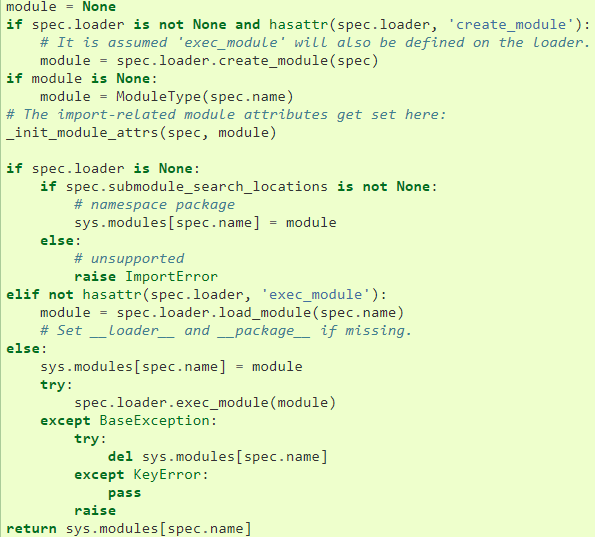
\includegraphics[scale=0.5]{import.png} \\
\begin{itemize}
\item 如果sys.modules中存在具有给定名称的现有模块对象,则import将返回它。
\item 如果sys.modules中存在具有给定名称的现有模块对象,则import将返回它。
\item 如果加载失败,则会从sys.modules中删除失败的模块 - 只有失败的模块。 sys.modules缓存中已有的任何模块以及作为副作用成功加载的任何模块都必须保留在缓存中。这与重新加载形成对比,即使故障模块仍留在sys.modules中。
\item 在创建模块之后但在执行之前,导入机制设置与导入相关的模块属性(上面的伪代码示例中的“_init_module_attrs”),如后面部分所述。
\item 模块执行是加载的关键时刻,模块的命名空间将被填充。执行完全委托给加载程序,加载程序可以决定填充的内容以及填充方式。
\item 在加载期间创建并传递给exec_module()的模块可能不是导入结束时返回的模块(importlib实现避免直接使用返回值。相反,它通过在sys.modules中查找模块名称来获取模块对象。这种间接影响是导入的模块可能会在sys.modules中替换自身。这是特定于实现的行为,不能保证在其他Python实现中起作用。)
\end{itemize}
\subsection{加载器loaders}
模块加载器提供了加载的关键功能:模块执行。导入机制使用\textbf{单个参数(要执行的模块对象)调用importlib.abc.Loader.exec_module()方法。从exec_module()返回的任何值都将被忽略。}\\
\indent 加载器必须满足以下要求:
\begin{itemize}
\item 如果模块是Python模块(与内置模块或动态加载的扩展相对),则加载器应在模块的全局名称空间(module.__dict__)中执行模块的代码。
\item 如果加载程序无法执行该模块,则应该引发ImportError,尽管在exec_module()期间引发的任何其他异常都将被传播。
\end{itemize}
在许多情况下,查找器和加载器可以是同一个物体;在这种情况下,find_spec()方法只返回一个规范,加载器设置为self。\\
\indent 模块加载器可以通过实现create_module()方法在加载期间选择创建模块对象。它需要一个参数,即module spec,并返回在加载期间使用的新模块对象。 create_module()不需要在模块对象上设置任何属性。如果方法返回None,则导入机制将自己创建新模块。\\
\indent 为了与现有的加载器兼容,导入机制将使用加载器的load_module()方法(注:该方法被3.4版本的exec_module方法替代)(如果存在且加载器也不实现exec_module())。但是,不推荐使用load_module(),而且加载器应该实现exec_module()。\\
\indent The load_module() method must implement all the boilerplate loading functionality described above in addition to executing the module. All the same constraints apply, with some additional clarification:
CHINESE (SIMPLIFIED)
除执行模块外,load_module()方法还必须实现上述所有样板加载功能。所有相同的限制条件都适用,并进一步澄清:
\begin{itemize}
\item 如果sys.modules中存在具有给定名称的现有模块对象,则加载程序必须使用该现有模块。 (否则,importlib.reload()将无法正常工作。)如果sys.modules中不存在指定的模块,则加载程序必须创建一个新的模块对象并将其添加到sys.modules。
\item 在加载程序执行模块代码之前,模块必须存在于sys.modules中,以防止无限制的递归或多次加载。
\item 如果加载失败,加载器必须删除已插入sys.modules的任何模块,但它必须\textbf{仅}删除失败的模块,并且仅当加载器本身已明确加载模块时。
\item Changed in version 3.6: An ImportError is raised when exec_module() is defined but create_module() is not.
\end{itemize}
\subsection{子模块}
当使用任何机制(例如importlib API,import或import-from语句或内置__import __())加载子模块时,绑定将放在父模块的命名空间中,并放到子模块对象中。例如,如果包spam具有子模块foo,则在导入spam.foo之后,spam将具有绑定到子模块的属性foo。假设您有以下目录结构:\\
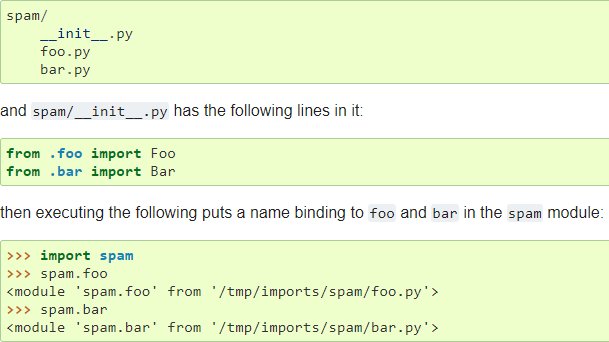
\includegraphics[scale=0.5]{submodule.png} \\
鉴于Python熟悉的名称绑定规则,这似乎令人惊讶,但它实际上是导入系统的基本功能。不变量保持是 如果你有sys.modules ['spam']和sys.modules ['spam.foo'](就像上面导入之后那样),后者必须显示为前者的foo属性。
\subsection{Module spec模块规格}
导入机制在导入期间使用有关每个模块的各种信息,尤其是在加载之前。大多数信息对所有模块都是通用的。模块规范的目的是基于每个模块封装此导入相关信息。\\
\indent 在导入期间使用规范允许在导入系统组件之间传输状态,例如,在创建模块规范的finder和执行它的loader之间。最重要的是,它允许导入机制执行装载的样板操作,而没有模块规格,loader有责任。\\
\indent 模块的规范在模块对象上公开为__spec__属性。有关模块规范内容的详细信息,请参阅\href{https://docs.python.org/3/library/importlib.html#importlib.machinery.ModuleSpec}{ModuleSpec}。
\subsection{导入相关的模块属性}
在加载程序执行模块之前,导入机制在加载期间根据模块的规范在每个模块对象上填充这些属性。
\paragraph{__name__}必须将__name__属性设置为模块的完全限定名称。此名称用于唯一标识导入系统中的模块。
\paragraph{__loader__}必须将__loader__属性设置为导入机制在加载模块时使用的加载程序对象。这主要用于内省,但可用于其他特定于加载程序的功能,例如获取与加载程序关联的数据。
\paragraph{__package__}必须设置模块的__package__属性。它的值必须是一个字符串,但它可以是与__name__相同的值。当模块是包时,其__package__值应设置为__name__。当模块不是包时,应将__package__设置为顶级模块的空字符串,或子模块的空字符串,设置为父包的名称。有关详细信息,请参阅PEP 366。\\
\indent 使用此属性代替__name__来计算主模块的显式相对导入,如PEP 366中所定义。它应与__spec__.parent具有相同的值。\\
\indent 在版本3.6中更改:__package__的值应与__spec__.parent相同
\paragraph{__spec__}
__spec__属性必须设置为导入模块时使用的模块规范。适当地设置__spec__同样适用于在解释器启动期间初始化的模块。一个例外是__main__,其中__spec__在某些情况下设置为None。\\
\indent 如果未定义__package__,则__spec__.parent将用作后备。\\
\indent 在版本3.6中更改:__spec__.parent在未定义__package__时用作后备。
\paragraph{__path__}
如果模块是包(常规或命名空间),则必须设置模块对象的__path__属性。该值必须是可迭代的,但如果__path__没有其他意义,则该值可能为空。如果__path__不为空,则迭代时必须生成字符串。有关__path__语义的更多细节\href{https://docs.python.org/3/reference/import.html#package-path-rules}{如下}。\\
\indent 非包模块不应具有__path__属性
\paragraph{__file__}
\paragraph{__cached__}__file__是可选的。如果设置,则此属性的值必须是字符串。如果导入系统没有语义含义(例如,从数据库加载的模块),则可以选择保留__file__。\\
\indent 如果设置了__file__,则设置__cached__属性也是合适的,该属性是代码的任何编译版本的路径(例如,字节编译文件)。设置此属性不需要存在该文件;路径可以简单地指向编译文件的存在位置(参见PEP 3147)。

\subsection{module.__path__} 
根据定义,如果模块具有__path__属性,则它是一个包。\\
\indent 在导入其子包期间使用包的__path__属性。在导入机制中,它的功能与sys.path非常相似。如,在导入期间提供搜索模块的位置列表。但是,__path__通常比sys.path更受限制。\\
\indent __path__必须是可迭代的字符串,但它可能是空的。用于sys.path的相同规则也适用于包的__path__,并且在遍历包的__path__时会查询sys.path_hooks(如下所述)。\\
\indent 包的__init__.py文件可以设置或更改包的__path__属性,这通常是在PEP 420之前实现命名空间包的方式。随着PEP 420的采用,命名空间包不再需要提供仅包含__init__.py的文件__path__操作代码;导入机制自动为命名空间包设置__path__。
\subsection{Module reprs}
默认情况下,所有模块都有一个可用的repr,但是根据上面设置的属性,在模块的规范中,您可以更明确地控制模块对象的repr。\\
\indent 如果模块具有规范(__spec__),则导入机制将尝试从其生成repr。如果失败或没有规范,导入系统将使用模块上可用的任何信息制作默认repr。它将尝试使用module.__ name__,module.__ file__和module.__ loader__作为repr的输入,默认情况下缺少任何信息。\\
以下是使用的确切规则:\\
\begin{itemize}
\item 如果模块具有__spec__属性,则使用规范中的信息生成repr。查阅“name”,“loader”,“origin”和“has_location”属性。
\item 如果模块具有__file__属性,则将其用作模块repr的一部分。
\item 如果模块没有__file__但是__loader__不是None,那么loader的repr用作模块repr的一部分。
\item 否则,只需在repr中使用模块的__name__。
\end{itemize}
\subsection{缓存的字节码失效(Cached bytecode invalidation)}
在Python从.pyc文件加载缓存的字节码之前,它会检查缓存是否与源.py文件一起是最新的。默认情况下,Python通过在写入时将源的最后修改时间戳和大小存储在缓存文件中来实现此目的。在运行时,import系统根据源的元数据检查缓存文件中存储的元数据来验证缓存文件。\\
\indent Python还支持“hash-based”的缓存文件,这些文件存储源文件内容的散列而不是其元数据。基于散列的.pyc文件有两种变体:checked and unchecked。\\
\indent 对于checked hash-based .pyc 文件,Python通过散列源文件并将生成的散列与缓存文件中的散列进行比较来验证缓存文件。如果发现checked hash-bashed 缓存文件无效,Python会重新生成它并写入新的checked hash-based 缓存文件。对于unchecked hash-bashed .pyc文件,Python只是假设如果缓存文件存在则其有效。hash-bashed .pyc文件验证行为可以使用--check-hash-based-pycs标志覆盖。\\
\indent 版本3.7中已更改:添加了基于散列的.pyc文件。以前,Python仅支持基于时间戳的字节码缓存失效。

\section{基于Path的查找器}
如前所述,Python附带了几个默认的元路径查找器。其中之一称为基于路径的查找程序(PathFinder),它会搜索导入路径(import path),其中包含路径条目列表(path entries)。每个路径条目都指定一个位置来搜索模块。\\
\indent 基于路径的查找器本身不知道如何导入任何东西。相反,它遍历各个路径条目,将每个条目与一个知道如何处理该特定路径的路径条目查找器相关联。(zx:分工明确,finder交由path entry处理)\\
\indent 默认的路径条目查找器集实现了在文件系统上查找模块的所有语义,处理特殊文件类型,如Python源代码(.py文件),Python字节代码(.pyc文件)和共享库(例如.so文件)。当标准库中的zipimport模块支持时,默认路径条目查找器还处理从zip文件加载所有这些文件类型(共享库除外)。\\
\indent 路径条目不必限于文件系统位置。它们可以引用URL,数据库查询或可以指定为字符串的任何其他位置。\\
\indent 基于路径的查找程序提供了额外的钩子和协议,以便您可以扩展和自定义可搜索路径条目的类型。例如,如果要将路径条目作为网络URL支持,则可以编写一个实现HTTP语义的钩子来在Web上查找模块。这个钩子(一个可调用的)将返回一个路径入口查找器,支持下面描述的协议,然后用于从Web获取模块的加载器。\\
\indent 警告:本节和前面两节都使用术语finder,通过使用术语meta path finder和path entry finder来区分它们。这两种类型的查找程序非常相似,支持类似的协议,并且在导入过程中以类似的方式运行,但重要的是要记住它们略有不同。特别是,元路径查找器在导入过程开始时运行,因为键入了\href{https://docs.python.org/3/library/sys.html#sys.meta_path}{sys.meta_path}遍历。\\
\indent 相比之下,路径入口查找器在某种意义上是基于路径的查找器的实现细节(zx:finder后需要entry来进入),事实上,如果要从sys.meta_path中删除基于路径的查找器,则不会调用任何路径条目查找器语义。
\subsection{Path entry finders}
path based finder负责查找和加载其模块的位置由字符串path entry指定的Python模块和软件包。大多数路径条目命名文件系统中的位置,但它们不必限于此。(zx:网络路径、数据库路径)\\
\indent 作为meta path finder,基于路径的查找器实现先前描述的find_spec()协议,但是它公开了可用于定制如何从导入路径找到和加载模块的其他钩子。\\
\indent path based finder,sys.path,sys.path_hooks和sys.path_importer_cache使用了三个变量。还使用包对象上的__path__属性。这些提供了可以定制进口机械的其他方式。\\
\indent sys.path包含一个字符串列表,提供模块和包的搜索位置。它是从PYTHONPATH环境变量和各种其他特定于安装和实现的默认值初始化的。sys.path中的条目可以命名文件系统上的目录,zip文件以及可能需要搜索模块的其他“位置”(请参阅​​站点模块),例如URL或数据库查询。 sys.path中只应包含字符串和字节;忽略所有其他数据类型。字节条目的编码由各个路径条目查找器确定。
\\indent path based finder是一个meta path finder,因此导入机制通过调用基于路径的finder的find_spec()方法开始导入路径搜索,如前所述。当给出find_spec()的path参数时,它将是一个要遍历的字符串路径列表 - 通常是该包中导入的包的__path__属性。\textbf{如果path参数为None,则表示使用顶级导入并使用sys.path。}\\
\indent path based finders遍历搜索路径中的每个条目,并为每个条目查找路径条目的相应路径条目查找器(PathEntryFinder)。因为这可能是昂贵的操作(例如,对于该搜索可能存在stat()调用开销),所以path based finder维护到路径条目查找器的高速缓存映射路径条目。此缓存在sys.path_importer_cache中维护(尽管名称如此,此缓存实际上存储finder objects,而不是importer objects(zx:指finder and loader对象))。以这种方式,对特定路径入口位置的path entry finder的昂贵搜索仅需要进行一次。用户代码可以从sys.path_importer_cache中删除缓存条目,强制基于路径的查找器再次执行路径条目搜索。\\
\indent 如果缓存中不存在path entry,则基于路径的查找程序将迭代sys.path_hooks中的每个可调用对象。列表中每一path entry hooks单一参数调用以搜索path entry。此可调用可以返回可以处理路径条目的path entry finder,也可以引发ImportError。path based finder使用ImportError来指示挂钩无法找到该路径条目的path entry finder。忽略该异常并继续导入路径迭代。钩子应该是一个字符串或字节对象;字节对象的编码取决于钩子(例如,它可能是文件系统编码,UTF-8或其他东西),如果钩子不能解码参数,它应该引发ImportError。\\
\indent 如果sys.path_hooks迭代以没有返回path entry finder结束,那么path based finder的find_spec()方法将在sys.path_importer_cache中存储None(表示该路径条目没有查找器)并返回None,表示这meta path finder找不到该模块。\\
\indent 如果sys.path_hooks上的某个path entry hooks可调用项返回path entry finder,则使用以下协议向finder询问module spec,然后在加载模块时使用该规范。\\
\indent 当前工作目录(由空字符串表示)的处理方式与sys.path上的其他条目略有不同。首先,如果发现当前工作目录不存在,则sys.path_importer_cache中不存储任何值。其次,每个模块查找都会查找当前工作目录的值。第三,用于sys.path_importer_cache并由importlib.machinery.PathFinder.find_spec()返回的路径将是实际的当前工作目录而不是空字符串。
\subsection{Path entry finder protocol}
为了支持模块和初始化包的导入以及为命名空间包提供部分,path  entry finders必须实现find_spec()方法。\\
\indent find_spec()接受两个参数,即要导入的模块的完全限定名称(foo.bar.some),以及(可选)目标模块。 find_spec()返回模块的完全填充规范。此规范将始终设置“loaders”(有一个例外(zx:__main__???))。

\section{替换标准导入系统}
替换整个导入系统的最可靠机制是删除sys.meta_path的默认内容,完全用自定义meta path hook替换它们。\\
\indent 如果只更改import语句的行为而不影响访问导入系统的其他API是可以接受的,那么替换builtin __import __()函数可能就足够了。此技术也可以在模块级别使用,以仅更改该模块中的import语句的行为。\\
\indent 要有选择地阻止在元路径的早期从hook导入某些模块(而不是完全禁用标准导入系统),直接从find_spec()引发ModuleNotFoundError就足够了而不是返回None。后者表示元路径搜索应该继续,而引发异常会立即终止它。
\section{__main__的特殊注意事项}
__main__模块是与Python的导入系统相关的特殊情况。如其他地方所述,__ main__模块在解释器启动时直接初始化,非常类似于sys和builtins。但是,与这两者不同,它并不严格限定为内置模块。这是因为初始化__main__的方式取决于调用解释器的标志和其他选项。
\subsection{__main__.__spec__}
据__main__的初始化方式,__main__.__ spec__被适当设置或设置为None。\\
\indent 当使用-m选项启动Python时,__spec__将设置为相应模块或包的module spec。当__main__模块作为执行目录,zipfile或其他sys.path entry的一部分加载时,也会填充__spec__。\\
\indent 在\href{https://docs.python.org/3/using/cmdline.html#using-on-interface-options}{the remaining cases}下,__main__.__spec__设置为None,因为用于填充__main__的代码与可导入模块不直接对应:
\begin{itemize}
\item interactive prompt(互动提示)
\item -c option
\item 从stdin运行
\item 直接从一个源文件或bytecode文件允许
\end{itemize}
请注意,__main__.__spec__在最后一种情况下始终为None,即使该文件在技术上可以直接作为模块导入。如果__main__中需要有效的模块元数据,请使用-m开关。\\
\indent 另请注意,即使__main__对应于可导入模块并且__main__.__spec__也相应地设置,它们仍然被视为(distinct)不同的模块。这是因为if __name__ ==“__ main__”保护的块:仅在模块用于填充__main__命名空间时执行,而不是在正常导入期间执行。














\end{document}